\documentclass[11pt]{article}
\usepackage[T1]{fontenc}
\usepackage[utf8]{inputenc}
\usepackage[a4paper,margin=25mm]{geometry}
\usepackage{amsmath,amssymb,amsthm}
\usepackage{tikz}
\usetikzlibrary{calc,positioning,arrows.meta}
\usepackage{hyperref,xurl}
\newtheorem{theorem}{Theorem}
\newtheorem{lemma}[theorem]{Lemma}
\newtheorem{proposition}[theorem]{Proposition}
\newtheorem{corollary}[theorem]{Corollary}
\theoremstyle{remark}
\newtheorem{remark}[theorem]{Remark}
\newcommand{\HH}{\mathbb H}
\newcommand{\ip}[2]{\langle #1,#2\rangle}
\newcommand{\Vol}{\operatorname{Vol}}
\title{Facet capacity and regular pentagons\linebreak
in compact right-angled hyperbolic four-polytopes}
\author{Coxeter Polytopes Frontier Project}
\date{24 October 2026}
\begin{document}
\maketitle

\begin{abstract}
Every compact right-angled hyperbolic four-polytope has at least $65$
facets and volume at least $49\pi^2/6$. The argument starts with a local
capacity inequality: a facet with $V$ vertices forces at least $2V+5$
facets in the ambient polytope. A maximum-distance projection supplies a
regular dodecahedral facet. We then exclude entire regular pentagons in
the small neighboring three-polyhedra, using two published fullerene
counts and explicit metric arguments. The same local geometry gives a
pentagon-excess gap $W=0$ or $W\ge17$; zero excess recognizes the regular
right-angled $120$-cell. We give the geometric arguments and the finite
verification algorithms separately. These results leave the absolute
minimum volume and the second compact volume open.
\end{abstract}

\section{Statement and scope}

Throughout, a polytope is convex and full-dimensional. A right-angled
hyperbolic polytope has dihedral angle $\pi/2$ at every ridge. All
polytopes in this paper are compact. In particular every edge has two
finite endpoints, and every two-face is a compact right-angled polygon.
If $P\subset\HH^4$, write $(v,e,r,f)$ for its numbers of vertices,
edges, ridges and facets.

\begin{theorem}\label{thm:global-lower}
Every compact right-angled hyperbolic four-polytope satisfies
\[
 f\ge65,\qquad \Vol(P)\ge\frac{49\pi^2}{6}.
\]
\end{theorem}

The proof has a shared geometric core and one finite branch. Actual
orthogonal walls control facet incidences, giving capacity and excess
inequalities. A spherical-code estimate then finds a regular dodecahedral
facet. Only at that point do we classify its possible small positive
neighbors: a $26$-vertex case and three $28$-vertex cases. Their complete
metric exclusions appear below. No arithmeticity or four-dimensional
polytope classification is assumed.

\begin{theorem}\label{thm:capacity}
Let $F$ be a facet of a compact right-angled hyperbolic four-polytope
$P$. If $F$ has $V$ vertices, then
\begin{equation}\label{eq:capacity}
 f\ge 2V+5.
\end{equation}
\end{theorem}

Define the pentagon excess by
\[
 W=\sum_{R\text{ a ridge of }P}\bigl(k(R)-5\bigr),
\]
where $k(R)$ is the number of sides of $R$. We will prove
\begin{equation}\label{eq:volume}
 W=v-5f,\qquad
 \Vol(P)=\frac{\pi^2}{12}(f+W+16).
\end{equation}
For a facet $F$, put
\[
 d(F)=\sum_{R\subset F}\bigl(k(R)-5\bigr).
\]
If it has $V$ vertices, then
\begin{equation}\label{eq:excess-identities}
 d(F)=\frac{V-20}{2},\qquad \sum_Fd(F)=2W.
\end{equation}

\begin{theorem}\label{thm:neighbor-excess}
Every facet with $V$ vertices satisfies
\begin{equation}\label{eq:excess-bound}
 W\ge\left\lceil\frac{3(V-20)}4\right\rceil,\qquad
 f+W\ge2V+5+\left\lceil\frac{3(V-20)}4\right\rceil
       \ge\frac{11V}4-10.
\end{equation}
\end{theorem}

\begin{corollary}\label{cor:local-size}
The following local size restrictions hold.
\begin{enumerate}
\item If $\Vol(P)\le34\pi^2/3$, every facet has at most $46$ vertices.
\item If $\Vol(P)<68\pi^2/3$, every facet has at most $96$ vertices.
\end{enumerate}
\end{corollary}

\begin{theorem}\label{thm:gap}
The pentagon excess satisfies $W=0$ or $W\ge17$. Moreover $W=0$ if
and only if $P$ is isometric to the regular right-angled $120$-cell.
\end{theorem}

The comparison values are the volumes of that $120$-cell and its facet
double. A distinct polytope at or below the first value must have
$W\ge17$ as well as the local cutoff $46$. The inequality
$f+W\ge120$ is still not proved. Neither universal minimality, a second
volume gap, nor decomposition into regular $120$-cells is assumed or
deduced.

The geometric input is the usual acute-chamber wall property: distinct
outward unit normals of an acute-angled hyperbolic polytope have
nonpositive scalar products. We use the standard Lorentz model and the
ordinary dual cell decomposition of the boundary of a simple convex
polytope. These are the acute-angle facts discussed in
\cite[pp.~63--64 and Proposition~4.1]{PV}, with the general geometric
background in~\cite{AVS}. We prove below the stronger compact normal gap,
the intersection and distinctness statements used in the count, and the
needed planar closing argument. The volume discussion also uses
Chern--Gauss--Bonnet for a compact hyperbolic reflection orbifold; its
resulting face formula agrees with~\cite[Proposition~3.2(d)]{KP}.
The capacity and neighboring-excess inequalities use no small-polyhedron
classification. The positive-excess gap and zero-excess recognition use
two further inputs, isolated in Section~\ref{sec:metric}: a compact
right-angled three-polyhedron with $12$ faces is the regular dodecahedron,
and the compact nonobtuse three-dimensional Andreev uniqueness theorem.
The later small-facet argument additionally uses the published fullerene
counts at $26$ and $28$ vertices, with their exact scope stated where they
enter. No classification or volume-minimum theorem in dimension four is an
input. Standard convex-polytope facts used below are Euler's formula,
the dual boundary sphere, and connectedness of facet adjacency.

The perpendicular-edge mechanism has an explicit antecedent in
Kellerhals--Perren's proof of Proposition~3.2(b), p.~1311~\cite{KP}:
the outgoing edges of a facet with $N$ vertices yield $N$ distinct
further facets. They use this to prove $f^2>4v$. Our count strengthens
that mechanism by controlling the extra facets needed around its
neighbors. The three-dimensional excess identity is already in
Inoue's Lemma~3.3~\cite{Inoue}. Neither that identity nor the
opposite-facet mechanism is claimed as new here.

\section{Normal geometry and perpendicular edges}

Use the hyperboloid model in $\mathbb R^{n,1}$, with scalar product of
signature $(-,+,\ldots,+)$. A point of $\HH^n$ is a future unit timelike
vector. An outward unit spacelike normal $a$ defines the half-space
$\ip{x}{a}\le0$.

\begin{lemma}\label{lem:gap}
Distinct wall normals of a compact right-angled polytope have product
either $0$ or strictly less than $-1$. A mutually orthogonal collection
of wall normals determines an actual common face.
\end{lemma}
\begin{proof}
Products are nonpositive by the acute-chamber wall property. Suppose
two normals $a,b$ have $g=\ip{a}{b}\in(-1,0)$. Their Gram matrix
\[
 G=\begin{pmatrix}1&g\\g&1\end{pmatrix}
\]
is positive definite and $G^{-1}$ has nonnegative entries. Let $p$ be a
strict future timelike interior point and set
$\beta=(\ip{p}{a},\ip{p}{b})^T<0$. The orthogonal projection
\[
 u=p-[a\ b]G^{-1}\beta
\]
adds nonnegative multiples of the outward normals to $p$. Thus it
strictly satisfies every other wall inequality. It satisfies the two
selected equalities, and
\[
 u^2=p^2-\beta^TG^{-1}\beta<0,\qquad
 \ip{p}{u}=u^2<0.
\]
It is therefore future timelike and gives an actual ridge, whose angle
is not $\pi/2$, a contradiction.

If $\ip{a}{b}=-1$, the nonzero vector $a+b$ is null. It has negative
product with $p$, hence is future. Its products with all other wall
normals are nonpositive. It would be a feasible ideal point, contrary
to compactness. The sum cannot be zero, because $p$ has negative product
with both summands. This proves the gap.

For mutually orthogonal normals $a_1,\ldots,a_j$, the same projection is
particularly simple:
\[
 u=p-\sum_{i=1}^j\ip{p}{a_i}a_i.
\]
It is future timelike, has zero product with each selected normal and
strict negative product with every other wall normal. Hence their
intersection is an actual codimension-$j$ face.
\end{proof}

At any finite vertex, all its incident normals lie in a positive definite
space. Lemma~\ref{lem:gap} makes them mutually orthogonal. There are
exactly $n$ of them, so the polytope is simple. A facet inherits right
angles: its neighboring wall normals are orthogonal to its own normal,
and serve as its intrinsic outward normals. The same applies to faces
of lower dimension. A compact right-angled $k$-gon has area
$(k-4)\pi/2>0$, so $k\ge5$.

\begin{lemma}\label{lem:footprint}
Fix a facet $A$ with normal $a$, and a facet disjoint from $A$ with
normal $z$. Any two common neighbors of these facets meet each other.
\end{lemma}
\begin{proof}
We have $\ip{a}{z}<-1$. The plane spanned by $a,z$ is Lorentzian, so
its orthogonal complement is positive definite. The normals $b,c$ of
two common neighbors belong to this complement. In a positive definite
space their product cannot be below $-1$. Product $-1$ would imply
$b=-c$, incompatible with a strict point of both negative half-spaces.
Lemma~\ref{lem:gap} therefore gives $\ip{b}{c}=0$, and the facets meet.
\end{proof}

We call the set of neighbors of $A$ meeting another facet its
\emph{footprint on the neighbors of $A$}. Lemma~\ref{lem:footprint}
says that a disjoint facet's footprint is a clique. This is the only
meaning of footprint used below.

\begin{lemma}\label{lem:opposite}
Let $A$ be a facet of a compact right-angled polytope in dimension three
or four. For every vertex $x$ of $A$, the edge leaving $A$ is perpendicular
to $A$ and ends on a facet $R_x$ disjoint from $A$. All the $R_x$ are
distinct. Moreover, $R_x$ meets a neighbor $B$ of $A$ if and only if $x$
belongs to $B$.

An actual facet disjoint from $A$ meeting all the neighbors of $A$ at
$x$ must be $R_x$.
\end{lemma}
\begin{proof}
Let $a$ be the outward normal of $A$. Regard $x$ as a vector in
$a^\perp$. Simplicity gives exactly one edge at $x$ not contained in
$A$. All its other defining walls are orthogonal to $a$, so its initial
direction is $-a$. If its length is $L_x>0$, the other endpoint is
\[
 y=\cosh(L_x)x-\sinh(L_x)a.
\]
The new normal there is forced to be
\begin{equation}\label{eq:opposite-normal}
 r_x=\sinh(L_x)x-\cosh(L_x)a.
\end{equation}
It is orthogonal to the walls defining the edge, has norm one and
satisfies $\ip{y}{r_x}=0$, $\ip{x}{r_x}<0$. Its product with $a$ is
$-\cosh(L_x)<-1$, so $R_x$ is disjoint from $A$.

For a neighbor $B$ with normal $b$,
\[
 \ip{r_x}{b}=\sinh(L_x)\ip{x}{b}.
\]
This is zero exactly when $x\in B$; the actual-intersection part of
Lemma~\ref{lem:gap} gives the stated incidence equivalence. If $r_x=r_y$,
projection to $a^\perp$ gives
$\sinh(L_x)x=\sinh(L_y)y$, hence $x=y$.

Finally a normal orthogonal to all the neighbors defining $x$ lies in
$\operatorname{span}(x,a)$. For an actual facet disjoint from $A$ its
orientation and its product with $x$ give the form
$r=\sinh(L)x-\cosh(L)a$, with $L>0$. Two distinct normals of this form
have product $\cosh(L-L_x)>0$, contrary to acuteness. Thus $r=r_x$.
\end{proof}

The final assertion is useful: a more distant wall on the same
perpendicular line cannot be counted as a second actual facet.

\section{Closing the neighborhood of a polygon}

\begin{lemma}\label{lem:polygon}
Let $Q\subset\HH^3$ be compact and right-angled, and let $A$ be a
$k$-gonal face. Then $Q$ has at least $2k+2$ faces. If it has exactly
$2k+2$, the unique face left after counting $A$, its $k$ neighbors and
its $k$ perpendicular-edge opposites is disjoint from all $k$ neighbors
of $A$.
\end{lemma}

\begin{proof}
Label the neighbors $A_1,\ldots,A_k$ cyclically. At the vertex where
$A_i$ and $A_{i+1}$ meet $A$, let $B_i$ be the opposite face supplied by
Lemma~\ref{lem:opposite}. Indices are cyclic. These are $1+2k$ distinct
faces. Among the $A_j$, the only neighbors of $B_i$ are $A_i,A_{i+1}$.
The $A_j$ themselves have just their cyclic adjacencies: any other
adjacency, together with $A$, would give an actual vertex of $A$ by
Lemma~\ref{lem:gap}.

Call any further face extra. Such a face meets at most one $A_i$.
Indeed two nonconsecutive $A_i$ cannot both meet it by
Lemma~\ref{lem:footprint}; meeting two consecutive ones would force it
to be the already counted $B_i$, by Lemma~\ref{lem:opposite}.

Pass to the dual triangulated two-sphere. Every vertex has degree at
least five, since every face of $Q$ is a compact right-angled polygon.
We use the elementary ear fact: a triangulated polygon with no interior
vertices has a vertex of degree two within that polygon. If one boundary
edge is prescribed, such an ear can be chosen away from its endpoints.
For example, root the tree dual to its triangles at that edge and take
a leaf away from the root; for a single triangle take the third vertex.

Suppose first there is no extra face. Each $A_i$ has exactly the five
known neighbors
\[
 A,\ A_{i-1},\ A_{i+1},\ B_{i-1},\ B_i.
\]
The cyclic link of $A_i$ forces the edge $B_{i-1}B_i$. The triangles
around $A$ and the $A_i$ form a disc whose complementary disc has boundary
$B_1,\ldots,B_k$ and no interior vertices. An ear in this disc has
degree two there, and has only its two outside neighbors $A_i,A_{i+1}$.
Its total degree would be four, a contradiction.

Now suppose there is exactly one extra face $C$, and it meets $A_i$.
It meets no other $A_j$. The five-neighbor argument still forces
$B_{j-1}B_j$ for $j\ne i$. At $A_i$ its cyclic link instead has the
segment $B_{i-1},C,B_i$. The complementary disc is therefore a polygon
with $C$ inserted into the $B$-cycle, again without interior vertices.
Every $B_j$ has just two outside $A$-neighbors, so needs degree at least
three within this disc. The vertex $C$ has just the outside neighbor
$A_i$, so needs degree at least four there. An ear is impossible. Hence
the unique extra face meets none of the $A_j$, as asserted.
\end{proof}

\begin{figure}[tb]
\centering
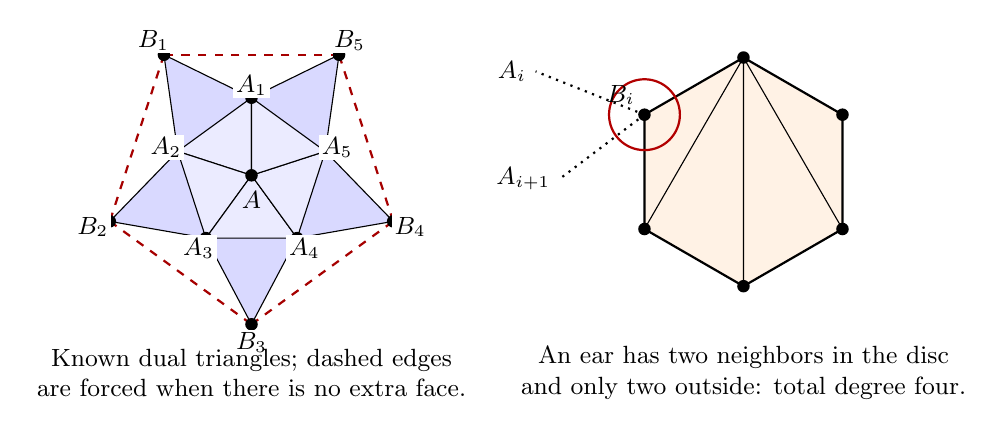
\begin{tikzpicture}[scale=.88,
  dot/.style={circle,fill=black,inner sep=1.6pt},
  every node/.style={font=\small}]
  \begin{scope}[xshift=-3.7cm]
    \coordinate (Z) at (0,0);
    \foreach \i in {1,...,5}{
      \pgfmathsetmacro{\ang}{90+72*(\i-1)}
      \pgfmathsetmacro{\bang}{126+72*(\i-1)}
      \coordinate (A\i) at (\ang:1.12);
      \coordinate (B\i) at (\bang:2.15);
    }
    \foreach \i in {1,...,5}{
      \pgfmathtruncatemacro{\j}{mod(\i,5)+1}
      \fill[blue!8] (Z)--(A\i)--(A\j)--cycle;
      \fill[blue!15] (A\i)--(B\i)--(A\j)--cycle;
      \draw (Z)--(A\i)--(A\j)--cycle;
      \draw (A\i)--(B\i)--(A\j);
      \draw[dashed,thick,red!65!black] (B\i)--(B\j);
    }
    \node[dot,label=below:$A$] at (Z) {};
    \foreach \i in {1,...,5}{
      \node[dot] at (A\i) {};
      \node[dot] at (B\i) {};
      \node[fill=white,inner sep=1pt] at ($(A\i)!-.16!(Z)$) {$A_{\i}$};
      \node[fill=white,inner sep=1pt] at ($(B\i)!-.12!(Z)$) {$B_{\i}$};
    }
    \node[align=center] at (0,-2.85)
      {Known dual triangles; dashed edges\\are forced when there is no extra face.};
  \end{scope}
  \begin{scope}[xshift=3.4cm,yshift=.05cm]
    \foreach \i in {0,...,5}{
      \pgfmathsetmacro{\ang}{90+60*\i}
      \coordinate (P\i) at (\ang:1.65);
    }
    \fill[orange!10] (P0)--(P1)--(P2)--(P3)--(P4)--(P5)--cycle;
    \draw[thick] (P0)--(P1)--(P2)--(P3)--(P4)--(P5)--cycle;
    \draw (P0)--(P2) (P0)--(P3) (P0)--(P4);
    \foreach \i in {0,...,5}{\node[dot] at (P\i) {};}
    \node[draw=red!70!black,circle,minimum size=9mm,thick] at (P1) {};
    \coordinate (U) at (-3.0,1.45);
    \coordinate (V) at (-2.65,-.1);
    \draw[dotted,thick] (P1)--(U) (P1)--(V);
    \node[left] at (U) {$A_i$};
    \node[left] at (V) {$A_{i+1}$};
    \node[above left] at (P1) {$B_i$};
    \node[align=center] at (0,-2.9)
      {An ear has two neighbors in the disc\\and only two outside: total degree four.};
  \end{scope}
\end{tikzpicture}
\caption{The dual closing argument. The left panel depicts the cyclic
incidences for $k=5$; the argument works for every $k\ge5$. The right
panel is a schematic triangulated complementary disc. These are
combinatorial drawings, not metric hyperbolic models.}
\label{fig:ear}
\end{figure}

The equality pattern can be recognized without a small-polyhedron list.
When there is exactly one extra face and it meets none of the $A_i$,
it is the unique interior vertex of the complementary $B$-disc. A chord
between two $B_i$ would cut off a polygon without this interior vertex.
The ear fact, applied away from that chord's endpoints, again gives a
$B_i$ of total degree four. Thus there are no chords and the extra face
joins every $B_i$. The result has two $k$-gons and two cyclic rows of
$k$ pentagons: the L\"obell face lattice. This agrees with the usual
description in~\cite[p.~17 of the author's version]{KK}. The capacity
argument uses only the proved disjointness of the extra face. The full
face lattice will also be used, with an explicit metric-uniqueness
input, in Section~\ref{sec:positive}.

\section{Capacity around a three-dimensional facet}

\begin{proof}[Proof of Theorem~\ref{thm:capacity}]
Let $F$ have $V$ vertices and $M$ two-faces. Trivalence and Euler's
formula inside $F$ give
\begin{equation}\label{eq:M}
 M=V/2+2.
\end{equation}
There are $M$ neighboring facets $F_1,\ldots,F_M$ and $V$ distinct
perpendicular-edge opposites $R_x$. Thus $1+M+V$ facets are already
counted. Call any other facet extra.

Suppose the ridge $F\cap F_i$ has $k_i$ sides. Inside $F_i$, the known
faces are precisely this ridge, its $k_i$ neighbors coming from the
other $F_j$, and its $k_i$ perpendicular-edge opposites coming from the
$R_x$ at its vertices. The perpendicular edges in $F_i$ are the same
edges of $P$ used in Lemma~\ref{lem:opposite}. If a different $F_j$
meets $F_i$, their three pairwise orthogonal normals with that of $F$
give an actual common edge by Lemma~\ref{lem:gap}; hence it is already
one of those $k_i$ neighbors. The opposite-incidence equivalence in
Lemma~\ref{lem:opposite} makes the list of $R_x$ exact as well.

Let $e_i$ count the further faces of $F_i$, all coming from extra
facets of $P$. Lemma~\ref{lem:polygon} gives $e_i\ge1$. An extra facet
has footprint at most two among the $F_j$. Indeed its footprint is a
clique by Lemma~\ref{lem:footprint}. Three members of this clique have
mutually orthogonal normals in the Lorentz space $a^\perp$ of signature
$(3,1)$, where $a$ is the normal of $F$. Together with $a$, they give
an actual vertex $x$ of $F$. A facet meeting all three is $R_x$, already
counted. A larger orthogonal collection cannot fit in $a^\perp$.

There is an additional restriction when $e_i=1$. The equality part of
Lemma~\ref{lem:polygon} says that its unique extra face is disjoint
from all the $k_i$ neighboring faces of $F\cap F_i$ inside $F_i$.
The parent extra facet cannot also meet another $F_j$: such a meeting
would force a common edge with $F_i,F_j$, contradicting that
disjointness. This extra facet therefore has singleton footprint
$\{i\}$.

Let $s$ be the number of indices with $e_i=1$. Their extra facets are
distinct and cannot serve any other index. The other $M-s$ indices
require at least $\sum_{e_i\ge2}e_i$ incidences. Since every remaining
extra facet serves at most two indices, the number of distinct extras
is at least
\[
 s+\frac12\sum_{e_i\ge2}e_i\ \ge\ s+(M-s)=M.
\]
Adding the previously counted facets and using~\eqref{eq:M} proves
\[
 f\ge1+M+V+M=2V+5.
\]
\end{proof}

\begin{figure}[tb]
\centering
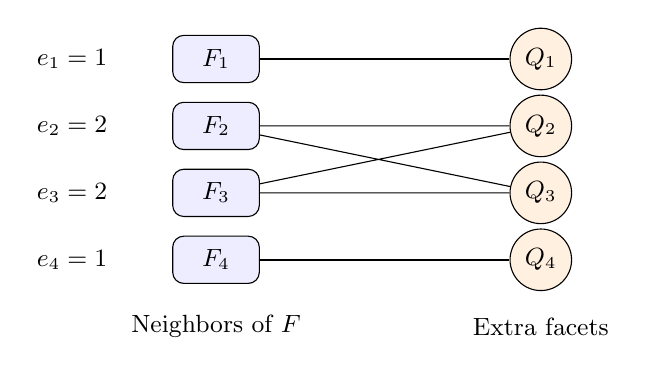
\begin{tikzpicture}[x=2.5cm,y=.85cm,
  face/.style={draw,rounded corners,fill=blue!7,minimum width=11mm,minimum height=6mm},
  extra/.style={draw,circle,fill=orange!12,inner sep=3pt},
  every node/.style={font=\small}]
  \foreach \i/\y in {1/3,2/2,3/1,4/0}{
    \node[face] (F\i) at (0,\y) {$F_{\i}$};
    \node[extra] (Q\i) at (1.65,\y) {$Q_{\i}$};
  }
  \draw[thick] (F1)--(Q1) (F4)--(Q4);
  \draw (F2)--(Q2) (F2)--(Q3) (F3)--(Q2) (F3)--(Q3);
  \node[left=7mm of F1] {$e_1=1$};
  \node[left=7mm of F2] {$e_2=2$};
  \node[left=7mm of F3] {$e_3=2$};
  \node[left=7mm of F4] {$e_4=1$};
  \node[align=center] at (0,-1.0) {Neighbors of $F$};
  \node[align=center] at (1.65,-1.0) {Extra facets};
\end{tikzpicture}
\caption{The final capacity count, shown as an incidence graph rather
than a claimed polytope realization. An index with $e_i=1$ consumes a
distinct singleton. Every other index needs at least two incidences,
while each remaining extra facet can serve at most two indices.}
\label{fig:capacity}
\end{figure}

\section{Pentagon excess and the volume reduction}

Because $P$ is simple, $e=2v$. Euler's formula for its boundary gives
$v-e+r-f=0$, hence $r=v+f$. At each vertex the link is a tetrahedron,
so six ridges meet there. Counting their corners yields
\[
 \sum_R k(R)=6v.
\]
It follows that
\[
 W=6v-5r=v-5f\ge0.
\]
Inside a facet $F$, trivalence gives $2E_F=3V$ and Euler gives
$M=V/2+2$. Therefore
\begin{equation}\label{eq:facet-excess}
 d(F)=3V-5M=\frac{V-20}{2}.
\end{equation}
Equivalently $d(F)=M-12$. Each ridge belongs to two facets, so
$\sum_Fd(F)=2W$. These identities also show that $d(F)\ge0$.

For completeness the compact volume formula can be recovered from the
reflection orbifold. The stabilizer of the interior of a codimension-$j$
face is a product of $j$ groups of order two. Its Euler characteristic
is consequently
\[
 \chi_{\mathrm{orb}}
 =1-\frac f2+\frac r4-\frac e8+\frac v{16}
 =\frac{v-4f+16}{16}.
\]
Chern--Gauss--Bonnet in dimension four gives
\[
 \Vol(P)=\frac{4\pi^2}{3}\chi_{\mathrm{orb}}
 =\frac{\pi^2}{12}(v-4f+16)
 =\frac{\pi^2}{12}(f+W+16),
\]
as in~\eqref{eq:volume}.

\begin{proof}[Proof of Theorem~\ref{thm:neighbor-excess}]
Let $F_1,\ldots,F_M$ be the distinct neighbors of $F$, and let
$F\cap F_i$ have $k_i$ sides. Lemma~\ref{lem:polygon} inside $F_i$
gives $d(F_i)\ge2k_i+2-12=2(k_i-5)$. Since
$\sum_i(k_i-5)=d(F)$, the nonnegative excesses of these distinct
facets satisfy
\[
 2W=\sum_Qd(Q)\ge d(F)+\sum_i d(F_i)\ge3d(F).
\]
Together with~\eqref{eq:facet-excess}, integrality and
Theorem~\ref{thm:capacity}, this proves~\eqref{eq:excess-bound}.
Shared ridges are allowed in the selected facet excesses: each is
counted twice in $\sum_Qd(Q)=2W$ as well. No disjointness of their
ridge contributions is being assumed.
\end{proof}

\begin{proof}[Proof of Corollary~\ref{cor:local-size}]
The regular right-angled $120$-cell has $v=600$, $f=120$ and $W=0$,
hence volume $34\pi^2/3$. In its double across a dodecahedral facet,
the $20$ common vertices cease to be vertices and the $12$ pairs of
neighboring facets merge. Thus $v=2\cdot600-2\cdot20=1160$,
$f=2\cdot120-2-12=226$ and $W=v-5f=30$, giving volume $68\pi^2/3$.
The first volume comparison is therefore $f+W\le120$. A facet with
$V=48$ already forces $f+W\ge101+21=122$ by
Theorem~\ref{thm:neighbor-excess}. Since its lower bound increases
with $V$ and $V$ is even, $V\le46$. Below the double,
$f+W<256$; $V=98$ would force $f+W\ge201+59=260$, so $V\le96$.
The endpoints $46$ and $96$ are not excluded by these calculations.
\end{proof}

\section{Metric inputs and the zero-excess case}\label{sec:metric}

We use the following two three-dimensional facts in the remaining
arguments, rather than include them in the capacity proof.
First, a compact right-angled three-polyhedron with $12$ faces,
equivalently $20$ vertices, is the regular right-angled dodecahedron;
see~\cite[Section~1.2]{ABVE}. Second, a fixed marked combinatorial
type with fixed nonobtuse dihedral angles has at most one compact
hyperbolic three-dimensional realization up to isometry, by the
uniqueness clause of~\cite[Theorem~1.4]{RHD}. The latter implies that
every combinatorial symmetry preserving the angles is realized by
an isometry. These are metric inputs; knowing only the face lattice
of a dodecahedron or a L\"obell polyhedron would not suffice.

\begin{proposition}\label{prop:zero}
$W=0$ if and only if $P$ is the regular right-angled $120$-cell.
\end{proposition}
\begin{proof}
The $120$-cell has pentagonal ridges, so its excess vanishes. Conversely
$W=0$ makes every facet have $d(F)=0$, hence $12$ faces. By the stated
three-dimensional classification every facet is a regular right-angled
dodecahedron.

Let $T$ be the regular right-angled $120$-cell. Match one whole facet
of $P$ isometrically with a facet of $T$, with their interiors on the
same inward side of its hyperplane. Take one of its pentagonal ridges
$R$. The normal plane to the hyperbolic plane spanned by $R$ is a
positive two-space. Once the normal of the matched facet is fixed,
there is a unique perpendicular normal line in it. Thus the facets
adjacent across $R$ in $P$ and $T$ have the same supporting hyperplane,
with the same inward orientation.

Inside that hyperplane, a regular dodecahedron containing the fixed
whole pentagon $R$ is unique on either side of $R$. Any two placements
differ by a symmetry of the regular pentagon, and those symmetries
extend to the regular dodecahedron. The inward side of the first
facet fixes the choice of side. Hence the adjacent whole facets agree.

Iterate across ridges. Connectedness of the facet graph of $P$ shows
that every facet of $P$ matches a facet of $T$. The nonempty matched
set is also closed under all neighbors in $T$, because every ridge
of a matched whole facet is already a ridge in $P$. Connectedness
of $T$'s facet graph gives every facet of $T$. Their supporting
halfspaces agree, so $P=T$.
\end{proof}

This uses regularity of \emph{every} facet. It does not propagate
from a single dodecahedral facet when its neighbors may be larger.

\section{Regular pentagons and positive facets}\label{sec:positive}

Call a facet \emph{positive} if $d(F)>0$. Define two graphs on the
positive facets. In $G$, an edge corresponds to a nonpentagonal ridge
and has positive integral weight $k-5$. In $H$, every adjacency of
positive facets is an edge, including pentagonal shared ridges. Thus
$G$ is a spanning subgraph of $H$. Its weighted degree at $F$ is
$d(F)$ and its total edge weight is $W$.

\begin{lemma}\label{lem:small-degree}
Every positive facet has $d(F)\ge2$. Graph $G$ has no vertex of
degree one. A degree-two vertex has equal edge weights $k-5$, its
facet is a L\"obell $L_k$, and $W\ge5k-15$.
\end{lemma}
\begin{proof}
A nonpentagonal ridge of size $k\ge6$ gives
$d(F)\ge2(k-5)\ge2$ by Lemma~\ref{lem:polygon}. More generally
an edge of weight $w$ gives $d(F)\ge2w$ at either endpoint, excluding
degree one. At degree two with weights $w_1,w_2$,
$w_1+w_2\ge2\max(w_1,w_2)$, so $w_1=w_2=w\ge1$.
Put $k=w+5$. The facet has exactly $2k+2$ faces, hence the
L\"obell type proved after Lemma~\ref{lem:polygon}: two disjoint
$k$-gonal bases and $2k$ lateral pentagons.

Its combinatorial $k$-fold rotation preserving both bases is realized
by an isometry, using the uniqueness input in Section~\ref{sec:metric}.
The convex base is therefore a regular right-angled $k$-gon. If $L_k$
is its edge length, the triangle from its center to a vertex to an
adjacent edge midpoint has angles $\pi/k,\pi/4,\pi/2$, giving
\begin{equation}\label{eq:regular-length}
 \cosh(L_k/2)=\sqrt2\cos(\pi/k),\qquad
 \cosh L_k=1+2\cos(2\pi/k).
\end{equation}
Write $L=L_5$, so $\cosh L=\phi=(1+\sqrt5)/2$. For $k\ge6$,
$L_k>L$. Each lateral pentagon contains a base edge of length $L_k$
and is consequently not a regular right-angled pentagon. Its other
facet neighbor cannot have zero excess, because every face of a
regular dodecahedron is a regular pentagon of edge length $L$.

All $2k$ lateral neighbors are therefore positive with excess at least
two. They and the two base neighbors are distinct: two convex facets
cannot share two different ridges. Each base neighbor has excess at
least $2(k-5)$. Including the original facet in the exact sum of
facet excesses gives
\[
 2W\ge2(k-5)+2\cdot2(k-5)+(2k)\cdot2=10k-30,
 \qquad W\ge5k-15\ge15.
\]
Only distinct facets were summed; their ridge contributions need not
be disjoint.
\end{proof}

\begin{lemma}\label{lem:loebell-six}
Every lateral pentagon of the right-angled L\"obell $L_6$ has cyclic
lengths $(b,a,c,c,a)$, with
\[
 \cosh b=2,\qquad \cosh a=\sqrt2,\qquad \cosh c=\sqrt3.
\]
Its edge on the hexagonal base is its unique longest edge.
\end{lemma}
\begin{proof}
Write the two bases as $U,D$ and the two lateral rows as $p_i,q_i$,
with indices modulo six. The neighbors of $p_i$ are
$U,p_{i-1},p_{i+1},q_{i-1},q_i$; those of $q_i$ are
$D,q_{i-1},q_{i+1},p_i,p_{i+1}$. The combinatorial reflection
$p_i\mapsto p_{-i}$, $q_i\mapsto q_{-i-1}$, fixing $U,D$,
is realized isometrically by three-dimensional uniqueness. It fixes
$p_0$ and exchanges its two $p$-neighbors and its two $q$-neighbors.
Its lengths therefore have the stated order, with $b$ on $U$.
Rotation and exchange of rows cover all lateral faces.

Equation~\eqref{eq:regular-length} gives $\cosh b=2$. For cyclic
lengths $s_i$ in a right-angled pentagon, the elementary identity is
\[
 \cosh(s_i)=\sinh(s_{i+2})\sinh(s_{i+3}).
\]
To derive it directly, put the common endpoint of sides $u=s_{i+2}$,
$v=s_{i+3}$ at $(1,0,0)$ in the Lorentz plane, with their outgoing
directions the two coordinate axes. The outward normals beyond their
far ends are $(\sinh u,\cosh u,0)$ and
$(\sinh v,0,\cosh v)$. Their product is $-\sinh u\sinh v$;
their connecting perpendicular is side $s_i$, so it also equals
$-\cosh(s_i)$. In the lateral pentagon this gives
$2=\sinh^2c$ and $\cosh a=\sinh c\sinh a$.
Hence $\cosh c=\sqrt3$, $\coth a=\sqrt2$ and $\cosh a=\sqrt2$.
Since $2>\sqrt3>\sqrt2$, the longest edge is unique.
\end{proof}

\begin{proposition}\label{prop:degree-two-twenty}
If $G$ has a degree-two vertex, then $W\ge20$.
\end{proposition}
\begin{proof}
For $k\ge7$ the preceding bound $W\ge5k-15$ suffices. Suppose
$k=6$, and call the original facet $F$, its two base neighbors
$B_1,B_2$, and their respective six lateral neighbors $A_{j,i}$,
$1\le i\le6$. These fifteen facets are distinct and each has
excess at least two, giving a baseline of thirty in $\sum d=2W$.

If $d(A_{j,i})=2$, then $A_{j,i}$ is also $L_6$: the edge-weight
inequality in Lemma~\ref{lem:small-degree} forces two unit edges.
Its shared pentagon with $F$ is lateral in both facets. Its unique
longest edge lies on $B_j$ when seen in $F$, and on a hexagonal
base when seen in $A_{j,i}$. These are the same edge. Exactly three
parent facets contain its interior, namely $F,A_{j,i},B_j$, by
compact simplicity. The hexagonal-base parent in $A_{j,i}$ must
therefore be $B_j$, since $F\cap A_{j,i}$ is pentagonal.
Thus $A_{j,i}$ and $B_j$ share a hexagon.

Let $m_j$ count the six lateral neighbors in row $j$ whose excess
exceeds two. Their excess above baseline is at least $m_j$.
The other $6-m_j$ give that many distinct unit $G$-edges at $B_j$,
in addition to $F B_j$. Consequently
\[
 d(B_j)-2\ge\max(0,5-m_j),\qquad
 m_j+\max(0,5-m_j)\ge5.
\]
The two rows and their bases are disjoint selected facet sets.
Adding their extra excesses to the baseline gives $2W\ge30+5+5=40$.
Other positive facets only increase this sum; no disjointness of
ridge contributions is assumed.
\end{proof}

\begin{lemma}\label{lem:three-edges}
A compact right-angled polygon with three consecutive edges of length
$L$ is the regular right-angled pentagon. In a nonpentagonal ridge
of $P$, three consecutive edges cannot all be carried by zero-excess
third facets.
\end{lemma}
\begin{proof}
Match the inward-oriented three-edge chain to three edges of the regular
right-angled pentagon. Fixed lengths and right-angle inward turns
determine the chain uniquely. At either end, the next supporting
line is the perpendicular through its endpoint. These two lines are
therefore the remaining two lines of the regular pentagon, with
the same inward orientations. They meet orthogonally. Crucially,
they are actual walls of the original polygon. The projection in
Lemma~\ref{lem:gap}, now in $\HH^2$, gives an actual finite vertex
at their intersection: all other wall inequalities stay strict.
Thus no further wall can truncate the putative closing vertex.
The boundary closes along those two lines, and the polygon is the
matched regular pentagon.

If an edge of a ridge $R=F\cap A$ is carried by a zero-excess third
facet $B$, it is an entire edge of the regular pentagon $F\cap B$
in the regular dodecahedron $B$. Its length is $L$. Apply the first
assertion to three such consecutive edges.
\end{proof}

\begin{figure}[tb]
\centering
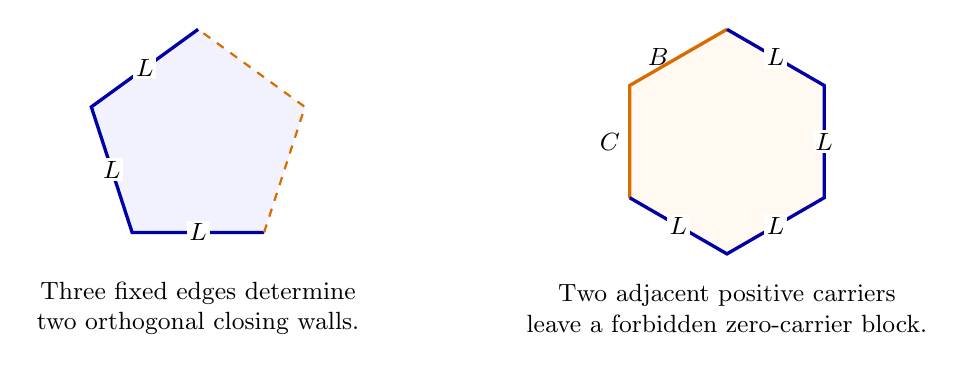
\begin{tikzpicture}[scale=.92,every node/.style={font=\small}]
 \begin{scope}[xshift=-3.7cm]
  \foreach \i in {0,...,4}{\coordinate (P\i) at ({90+72*\i}:1.55);}
  \fill[blue!5] (P0)--(P1)--(P2)--(P3)--(P4)--cycle;
  \draw[very thick,blue!65!black] (P0)--(P1)--(P2)--(P3);
  \draw[dashed,thick,orange!85!black] (P3)--(P4)--(P0);
  \foreach \i/\j in {0/1,1/2,2/3}{
   \path (P\i)--node[fill=white,inner sep=1pt] {$L$} (P\j);}
  \node[align=center] at (0,-2.3)
   {Three fixed edges determine\\two orthogonal closing walls.};
 \end{scope}
 \begin{scope}[xshift=3.6cm]
  \foreach \i in {0,...,5}{\coordinate (Q\i) at ({90+60*\i}:1.55);}
  \fill[orange!5] (Q0)--(Q1)--(Q2)--(Q3)--(Q4)--(Q5)--cycle;
  \draw[very thick,orange!85!black] (Q0)--(Q1)--(Q2);
  \draw[very thick,blue!65!black] (Q2)--(Q3)--(Q4)--(Q5)--(Q0);
  \foreach \i/\j in {2/3,3/4,4/5,5/0}{
   \path (Q\i)--node[fill=white,inner sep=1pt] {$L$} (Q\j);}
  \node[left] at ($(Q0)!.5!(Q1)$) {$B$};
  \node[left] at ($(Q1)!.5!(Q2)$) {$C$};
  \node[align=center] at (0,-2.3)
   {Two adjacent positive carriers\\leave a forbidden zero-carrier block.};
 \end{scope}
\end{tikzpicture}
\caption{The polygon obstruction. Blue edges have the regular-pentagon
length $L$. In the right panel, a nonpentagonal ridge with only the
two adjacent positive carriers $B,C$ would have at least four consecutive
blue edges. The drawings show the boundary order, not Euclidean
representations of the hyperbolic right angles.}
\label{fig:pentagon-chain}
\end{figure}

For a positive facet $F$, let $J_F$ be the graph induced by $H$ on
its neighbors. Its vertices are the positive facets meeting $F$.
Call a vertex of $J_F$ \emph{eligible} if its degree is at least three,
or if its degree is two and its two neighbors are not adjacent.

\begin{lemma}\label{lem:eligibility}
Every $G$-neighbor of $F$ is eligible in $J_F$.
\end{lemma}
\begin{proof}
For a nonpentagonal ridge $R=F\cap A$, the degree of $A$ in $J_F$
is exactly its number of positive third-facet edge carriers. A common
neighbor gives an actual edge of $R$ by projection of three orthogonal
normals. If there are at most one such carrier, its other at least
$k-1\ge5$ edges form a consecutive zero-carrier block, contradicting
Lemma~\ref{lem:three-edges}. If there are exactly two and they are
adjacent in $J_F$, projection of four orthogonal normals gives an
actual common vertex in $R$. Their edges are adjacent; the remaining
$k-2\ge4$ consecutive edges are zero-carried, again impossible.
\end{proof}

\begin{lemma}\label{lem:four-graph}
A graph on at most four vertices with no $K_4$ and no induced $C_4$
has at most two eligible vertices.
\end{lemma}
\begin{proof}
If it has a degree-three vertex, the remaining three vertices induce
zero, one or two edges; three would give $K_4$. With zero or one,
only the degree-three vertex can be eligible. With two, they form a
path. Its middle and the original vertex have degree three, while
each endpoint has two adjacent neighbors and is ineligible. If there
is no degree-three vertex, all components are paths or cycles.
Triangles have no eligible vertex, $C_4$ is excluded, and a path on
at most four vertices has at most two internal vertices.
\end{proof}

\begin{corollary}\label{cor:min-degree}
If $G$ has minimum degree at least three, then $H$ has minimum degree
at least five. In particular both conclusions hold when $0<W<20$.
\end{corollary}
\begin{proof}
The assertion about $G$ when $0<W<20$ follows from
Lemma~\ref{lem:small-degree} and Proposition~\ref{prop:degree-two-twenty}.
Assume now that $G$ has minimum degree at least three. If a positive
facet $F$ had at most four $H$-neighbors, $J_F$ would have at least
three eligible vertices by Lemma~\ref{lem:eligibility}. It has no
$K_4$, since together with $F$ that would give five orthogonal unit
normals in signature $(4,1)$. It has no induced $C_4$: the two
nonadjacent pairs in such a square would be orthogonal Lorentzian
normal planes, giving two negative directions. Equivalently apply
Lemma~\ref{lem:footprint} to either disjoint pair. Thus
Lemma~\ref{lem:four-graph} gives a contradiction.
\end{proof}

\section{The small-graph obstruction}

\begin{lemma}\label{lem:nine}
A graph $C$ on nine vertices with maximum degree at most three and
no induced pair of disjoint edges has an independent set of size five.
\end{lemma}
\begin{proof}
Suppose first it contains a triangle $T$. Its vertices have only three
degree slots outside $T$ in total. Partition the other six vertices
into $D$, those having a neighbor in $T$, and $S$, those having none.
Then $|D|\le3$, $|S|\ge3$. Set $S$ is independent, because an edge
in $S$ with a triangle edge would induce two disjoint edges. If
$|S|\ge4$, add any triangle vertex.

Otherwise $|S|=|D|=3$, and all three slots are used, as a perfect
matching from $T$ to $D$. There is no $D$--$S$ edge: such an edge
and the triangle edge avoiding its $D$-endpoint's unique neighbor
would induce two disjoint edges. Thus $S$ consists of three isolated
vertices. A triangle vertex and a $D$-vertex matched to a different
triangle vertex are independent. With $S$ they give five.

Suppose now $C$ is trianglefree. If it is bipartite, one independent
part has at least five vertices. Otherwise a shortest odd cycle is
induced. Its length is five, since any induced cycle of length at
least six contains an induced pair of disjoint edges. Write this
cycle as $T=(t_0,\ldots,t_4)$.

Each cycle vertex has at most one outside neighbor, so there are at
most five contacts to the other four vertices. An outside vertex has
at most two cycle neighbors, nonadjacent by trianglefreeness. It
cannot have exactly one, say $t_i$: its edge to $t_i$ and the cycle
edge $t_{i+2}t_{i+3}$ would induce two disjoint edges. Thus outside
vertices have zero or two cycle neighbors, and at least two have zero.
Each zero-contact vertex $d$ is isolated. For if $de$ were an outside
edge, the at most two cycle neighbors of $e$ cannot cover all cycle
edges; an uncovered cycle edge with $de$ is forbidden.

If there are at least three isolated vertices, add two independent
cycle vertices. If exactly two, take another outside vertex $e$.
Deleting its two nonadjacent cycle neighbors leaves three cycle
vertices with an independent pair. That pair, $e$ and the two
isolated vertices form an independent five.
\end{proof}

\begin{figure}[tb]
\centering
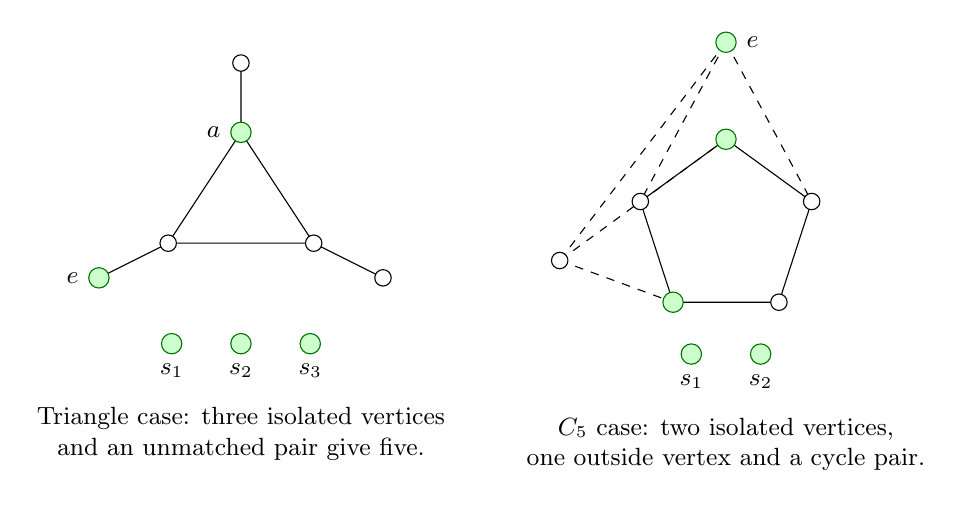
\begin{tikzpicture}[scale=.88,
 dot/.style={circle,draw,fill=white,inner sep=2.1pt},
 chosen/.style={circle,draw=green!45!black,fill=green!20,inner sep=2.6pt},
 every node/.style={font=\small}]
 \begin{scope}[xshift=-3.5cm]
  \coordinate (A) at (0,1.4);\coordinate (B) at (-1.05,-.2);
  \coordinate (C) at (1.05,-.2);
  \coordinate (D) at (0,2.4);\coordinate (E) at (-2.05,-.7);
  \coordinate (F) at (2.05,-.7);
  \draw (A)--(B)--(C)--cycle (A)--(D) (B)--(E) (C)--(F);
  \node[chosen,label=left:$a$] at (A) {};
  \node[dot] at (B) {};\node[dot] at (C) {};
  \node[dot] at (D) {};\node[chosen,label=left:$e$] at (E) {};
  \node[dot] at (F) {};
  \foreach \i/\x in {1/-1,2/0,3/1}{
   \node[chosen,label=below:$s_{\i}$] at (\x,-1.65) {};}
  \node[align=center] at (0,-2.95)
   {Triangle case: three isolated vertices\\and an unmatched pair give five.};
 \end{scope}
 \begin{scope}[xshift=3.5cm]
  \foreach \i in {0,...,4}{\coordinate (T\i) at ({90+72*\i}:1.3);}
  \draw (T0)--(T1)--(T2)--(T3)--(T4)--cycle;
  \coordinate (U) at (0,2.7);\coordinate (V) at (-2.4,-.45);
  \draw[dashed] (U)--(T1) (U)--(T4) (V)--(T0) (V)--(T2) (U)--(V);
  \node[chosen,label=right:$e$] at (U) {};
  \node[dot] at (V) {};
  \node[chosen] at (T0) {};\node[chosen] at (T2) {};
  \foreach \i in {1,3,4}{\node[dot] at (T\i) {};}
  \node[chosen,label=below:$s_1$] at (-.5,-1.8) {};
  \node[chosen,label=below:$s_2$] at (.5,-1.8) {};
  \node[align=center] at (0,-3.1)
   {$C_5$ case: two isolated vertices,\\one outside vertex and a cycle pair.};
 \end{scope}
\end{tikzpicture}
\caption{Independent sets in Lemma~\ref{lem:nine}, highlighted in green.
Only contacts used in the argument are shown. Additional edges among
the unselected outside vertices do not affect the highlighted set;
these are diagrams of the proof cases, not polytope realizations.}
\label{fig:nine}
\end{figure}

\begin{proposition}\label{prop:ten-positive}
If $G$ has minimum degree at least three, there are at least ten
positive facets.
\end{proposition}
\begin{proof}
Let $N$ be the number of positive facets, and suppose $N\le9$.
Corollary~\ref{cor:min-degree} gives minimum degree five in $H$.
Let $C$ be the complement of $H$. It has no independent five, since
$H$ has no $K_5$, and no induced pair of disjoint edges, since $H$
has no induced square. Its maximum degree is at most $N-6$.

For $N\le5$, minimum degree five in $H$ is impossible; $N=6$
would give $H=K_6$. For $N=7$, $C$ has maximum degree one and at
most one edge, since two would form a forbidden induced pair.
It therefore has an independent set of size at least six.

For $N=8$, maximum degree in $C$ is two. At most one component
can contain an edge. That component is a path on at most four
vertices or a cycle on at most five: longer paths or cycles contain
an induced pair of disjoint edges. The path cases, together with
isolated vertices, give an independent set of size at least six.
Cycles of lengths three, four and five give independent sets of
sizes six, six and five respectively. Finally $N=9$ is excluded by
Lemma~\ref{lem:nine}. All cases contradict the absence of an
independent five, proving $N\ge10$.
\end{proof}

The proof uses $H$, not just $G$, when excluding induced squares.
A diagonal of $G$ might be a pentagonal adjacency and hence present
in $H$; it cannot be discarded from the normal geometry.

\section{Five-neighbor links and the positive-excess gap}\label{sec:endpoint}

For the remaining small-excess cases we need the exceptional edge lengths,
not only the number of positive carriers. We first record two
elementary polygon facts.

\begin{lemma}\label{lem:pentagon-two}
A compact right-angled pentagon with two adjacent edges of length $L$
is regular. In particular it is regular if any three edges have length $L$.
\end{lemma}
\begin{proof}
Match the two-edge chain to the regular pentagon. This fixes its three
vertices and the perpendicular supporting lines through its two outer
endpoints. These lines are ultraparallel, as in the regular model.
The remaining fifth side is their unique common perpendicular, fixing
the entire pentagon. Among any three edges of a pentagon two are
adjacent, giving the second assertion.
\end{proof}

\begin{lemma}\label{lem:hexagon-four}
Suppose four specified edges of a compact right-angled hexagon have
length $L$. Its other two side positions are opposite, and both
remaining lengths are $2L$.
\end{lemma}
\begin{proof}
Otherwise three of the four fixed positions are consecutive, contrary
to Lemma~\ref{lem:three-edges}. Write the cyclic lengths as
$a,L,L,d,L,L$ and put $A=\cosh a$, $D=\cosh d$, $p=\cosh L=\phi$.
The right-angled hexagon relations are
\[
 A=\frac{p^2+D}{p^2-1},\qquad D=\frac{p^2+A}{p^2-1}.
\]
They also have a short direct Lorentz derivation. For cyclic sides
$a,b,c,d,e,f$, let $x,y$ be the future unit endpoints of $a$ and
$n_a$ its outward normal. The outward normals of $c,e$ are
\[
 n_c=\sinh(b)x-\cosh(b)n_a,\qquad
 n_e=\sinh(f)y-\cosh(f)n_a.
\]
Their product is
$\cosh(b)\cosh(f)-\cosh(a)\sinh(b)\sinh(f)=-\cosh(d)$:
the connecting perpendicular is side $d$. This gives the first
relation and, on exchanging opposite sides, the second.
Since $p^2-1=p$, subtraction gives $A=D$, and
\[
 A=D=\frac{p^2}{p-1}=p^3=\cosh(2L).
\]
The lengths are positive, so both equal $2L$.
\end{proof}

\begin{lemma}\label{lem:five-neighbor-exclusion}
If $G$ has minimum degree at least three, a facet of excess three
cannot have exactly five positive neighbors.
\end{lemma}
\begin{proof}
Suppose $d(F)=3$ and $F$ has five positive neighbors. Its weighted
$G$-degree and minimum unweighted degree force exactly three unit
edges. It therefore has three hexagons and twelve pentagons.
Put $J=J_F$. Its five vertices
represent the positive neighbor faces of $F$; mark the three
hexagons. Graph $J$ has no $K_4$ and no induced $C_4$. Every other
face of $F$ borders a zero-excess facet, so is a regular pentagon.
Thus every edge of a marked hexagon whose carrier is absent from
$J$ has length $L$. Actual edge and vertex intersections follow
from Lemma~\ref{lem:gap}; graph adjacencies are not merely formal.

A marked vertex has degree at least two. At degree two,
Lemma~\ref{lem:hexagon-four} forces its neighbors to be nonadjacent
and its two carrier edges to be opposite, both of length $2L$.
At degree three, its neighbor graph cannot be a three-vertex path:
that would place its three positive carrier edges consecutively
in the hexagon, leaving three consecutive $L$-edges, contrary to
Lemma~\ref{lem:three-edges}. A triangle among its neighbors is
already excluded by the absence of $K_4$. We now exhaust $J$.

If $J$ has a universal vertex $v$, its other four vertices induce
a trianglefree graph with no induced square, hence a forest $B$.
A $B$-degree-zero vertex has $J$-degree one and is unmarked.
A $B$-degree-one vertex has two adjacent $J$-neighbors and is
unmarked. A $B$-degree-two vertex has three $J$-neighbors forming
a path centered at $v$, and is unmarked. Only a $B$-degree-three
vertex remains eligible for a mark, and a four-vertex forest has
at most one. Including $v$ gives at most two marks, a contradiction.

We may therefore assume $J$ has maximum degree three. Suppose
it contains a triangle $T$, with outside vertices $d,e$. If $de$
is absent, an outside vertex with zero or one $T$-contact has
degree at most one; with two contacts its degree-two neighbors
are adjacent; three contacts give $K_4$. Neither outside vertex
can be marked. A marked triangle vertex must have a unique
outside contact, and that outside vertex must contact no other
triangle vertex: otherwise its three neighbors form a path.
There are only two outside vertices, so at most two marks.

If $de$ is present, let $D,E\subset T$ be their contact sets.
They are disjoint, since a common triangle neighbor would have
degree four. They are nested, since $x\in D\setminus E$ and
$y\in E\setminus D$ give an induced square $x,d,e,y$.
Thus one set is empty; say $E=\varnothing$, and $|D|\le2$.
If $D$ is empty there are no marks. If $|D|=1$, only $d$ and
its triangle neighbor can be marked. If $|D|=2$, only $d$ can
be marked: its triangle neighbors have three-neighbor paths,
while the remaining triangle vertex has two adjacent neighbors.
In all cases $e$ has degree one. Thus no graph containing a
triangle has three marks.

Finally suppose $J$ is trianglefree. It is a forest or $C_5$:
any cycle has length five, and a chord would create a triangle.
A forest on five vertices with at least three vertices of degree
at least two must be $P_5$, with its three internal vertices
marked. Each marked hexagon has degree two and its carrier
edges have length $2L$. An endpoint of $P_5$ represents a
pentagon, with four zero-carried $L$-edges. It is regular by
Lemma~\ref{lem:pentagon-two}, contradicting the shared $2L$-edge.
In $C_5$ the three marked hexagons again have $2L$ carrier
edges. One of the other two vertices is adjacent to a marked
vertex. Its pentagon has three zero-carried $L$-edges, so is
regular by the same lemma; its shared $2L$-edge is impossible.
Every possible $J$ has been excluded, proving the local assertion.
\end{proof}

The local proof needs the marked polygon geometry. The weaker
abstract conditions on ten vertices alone are consistent: the graph
$C_5[K_2]$, obtained by replacing each cycle vertex by an adjacent
pair and joining consecutive pairs completely, has minimum degree
five, no $K_5$ and no induced $C_4$. We have not excluded it by
an unsupported small-graph assertion.

\begin{lemma}\label{lem:ten-complement}
Let $C$ have ten vertices, no induced pair of disjoint edges, and
maximum degree at most four. If at most two vertices have degree
four, then $C$ has an independent set of size five.
\end{lemma}
\begin{proof}
If at most one vertex has degree four, delete it, or any vertex if
there is none. The remaining nine-vertex graph is subcubic, so
Lemma~\ref{lem:nine} applies. If two degree-four vertices $u,v$
are adjacent, deleting $u$ again leaves a subcubic graph.

It remains to treat nonadjacent degree-four vertices $u,v$. Set
\[
 X=N(u)\cap N(v),\quad t=|X|,\quad
 A=N(u)\setminus N(v),\quad B=N(v)\setminus N(u),
\]
and let $S$ consist of the other vertices adjacent to neither $u$ nor $v$.
These partition the other eight vertices, with
$|A|=|B|=4-t$ and $|S|=t$. All these vertices have degree at most
three. Every $a\in A$ meets every $b\in B$, since otherwise
$ua,vb$ induce two disjoint edges. If $A$ is nonempty, its vertices
have degree at least $1+(4-t)$, so $t\ge2$. Thus $t=2,3,4$.

An edge $yz$ in $S$ must collectively contact every vertex of
$N(u)\cup N(v)$: an uncovered $x\in N(u)$ would give the induced
pair $yz,ux$, and similarly for $v$. Its endpoints have at most
four spare degrees after $yz$. For $t=2,3$ the union has six or
five vertices, respectively, so $S$ is independent.

At $t=2$, the two-element sets $A,B$ are saturated by their
complete cross contacts and their respective $u,v$ contacts.
Thus $A$ is independent and has no $S$ contacts. The set
$\{v\}\cup A\cup S$ is an independent five. At $t=3$, simply
take $\{u,v\}\cup S$.

At $t=4$, $A=B=\varnothing$. An $S$-edge $yz$ must use all
four spare degrees on the four vertices of $X$. Neither endpoint
can have another $S$-neighbor. Any second $S$-edge would then
induce two disjoint edges with $yz$. Hence $S$ has at most one
edge and an independent triple. Together with $u,v$ this gives five.
\end{proof}

\begin{proof}[Proof of Theorem~\ref{thm:gap}]
The zero case is Proposition~\ref{prop:zero}. Suppose $0<W\le16$.
By Proposition~\ref{prop:degree-two-twenty} and
Lemma~\ref{lem:small-degree}, graph $G$ has minimum degree at
least three. Let $N$ be its number of vertices and $E$ its
unweighted edge count. Then
\[
 3N\le2E\le2W\le32.
\]
Proposition~\ref{prop:ten-positive} gives $N\ge10$, so $N=10$.
Each positive facet has excess at least three, and the total excess
is at most thirty-two. Thus at most two of them have excess greater
than three. By Lemma~\ref{lem:five-neighbor-exclusion}, every
other facet has $H$-degree at least six; the exceptional two have
degree at least five by Corollary~\ref{cor:min-degree}.

The complement $C$ of $H$ therefore has maximum degree four,
with at most two vertices of degree four. It has no induced pair
of disjoint edges because $H$ has no induced square.
Lemma~\ref{lem:ten-complement} gives an independent five in $C$,
a forbidden $K_5$ in $H$. This contradiction excludes all
$0<W\le16$ at once, proving the theorem.
\end{proof}


\section{A dodecahedron among the farthest facets}\label{sec:farthest}

We next find the regular facet which starts the small-neighbor argument.
The distance in this section is to a supporting hyperplane. Acuteness
keeps its orthogonal projection in the actual facet, as the wall check
below shows. Maximization then bounds all the intrinsic neighboring
heights at once.

\begin{theorem}\label{thm:farthest-dodecahedron}
Let $q$ be an interior point of $P$, and put
\[
 t_n=-\ip qn,\qquad T=\max_n t_n,
 \qquad \phi=(1+\sqrt5)/2,
\]
where $n$ ranges over the outward unit facet normals. Every facet
attaining $T$ is a regular right-angled dodecahedron. Moreover
$T^2\ge\phi^3$, with equality exactly for the regular right-angled
$120$-cell at its center.
\end{theorem}
\begin{proof}
Choose a maximizing normal $n$. The point
\[
 q'=\frac{q+Tn}{\sqrt{1+T^2}}
\]
is future unit timelike and lies on its wall. For every other actual
normal $m$, acuteness gives
\[
 \ip{q'}m=\frac{\ip qm+T\ip nm}{\sqrt{1+T^2}}<0.
\]
Thus $q'$ lies in the relative interior of the actual facet $F$.
Its intrinsic normals are precisely the parent normals $m_i$ adjacent
to $F$, and their intrinsic heights satisfy
\[
 0<t'_i=\frac{t_{m_i}}{\sqrt{1+T^2}}
       \le\frac{T}{\sqrt{1+T^2}}<1.
\]
In intrinsic Lorentz coordinates centered at $q'$, write
$m_i=(t'_i,\sqrt{1+t_i'^2}\,u_i)$ with $u_i\in S^2$.
Their distinct directions obey
\[
 u_i\cdot u_j\le
 \frac{t'_it'_j}{\sqrt{(1+t_i'^2)(1+t_j'^2)}}<\frac12.
\]

Here a small polynomial bound suffices. Set
\[
 f(x)=(x+1)(x+2/5)^2(x-1/2).
\]
It is nonpositive on $[-1,1/2]$, and its Legendre expansion is
\[
 f=\frac7{50}P_0+\frac{23}{50}P_1+\frac{107}{175}P_2
       +\frac{13}{25}P_3+\frac8{35}P_4,
 \qquad f(1)=\frac{49}{25}.
\]
We recall directly why the four nonconstant kernels have nonnegative
ordered-pair sums. For a unit vector $u\in\mathbb R^3$, the trace-free
symmetric tensors
\[
 \begin{split}
 A_2(u)&=u^2-I/3,\\
 A_3(u)&=u^3-\operatorname{sym}_3(uI)/5,\\
 A_4(u)&=u^4-\operatorname{sym}_6(u^2I)/7
                       +\operatorname{sym}_3(II)/35
 \end{split}
\]
have contraction kernels
\[
 x^2-1/3,\qquad x^3-3x/5,\qquad x^4-6x^2/7+3/35.
\]
The symmetrizations are the unnormalized sums over the indicated
distinct positions; $u^j$ denotes a tensor power and $I$ the Euclidean
metric tensor. For example, tracing $A_4$ gives
$u^2-(7u^2+I)/7+5I/35=0$; contraction with a trace-free tensor
then removes its trace terms. These kernels are positive multiples of
$P_2,P_3,P_4$. Their ordered-pair sums are squared tensor-sum norms;
the same statement for $P_1$ is the ordinary squared vector-sum norm.
If there are $N$ directions, it follows that
\[
 \frac7{50}N^2\le\sum_{i,j}f(u_i\cdot u_j)
                    \le\frac{49}{25}N.
\]
Thus $N\le14$. At $N=14$ every off-diagonal term must vanish.
Strict separation excludes the root $1/2$, so all pair products would
be $-1$ or $-2/5$. But then
\[
 \Bigl\|\sum_i u_i\Bigr\|^2
 \le N-\frac25N(N-1)<0.
\]
Hence $N\le13$.

By Lemma~\ref{lem:polygon}, a compact right-angled three-polyhedron
with at most thirteen faces has no face of size at least six. Every
face is pentagonal, and Euler gives exactly twelve faces. The metric
input of Section~\ref{sec:metric} makes $F$ the regular dodecahedron.
This applies to every maximizing $n$.

To obtain the stated radius, put the intrinsic center of that
dodecahedron at $(1,0)$. Its twelve normals are
$(h,\sqrt{1+h^2}\,r_i)$, where the $r_i$ are the regular icosahedral
directions. Adjacent directions have product $1/\sqrt5$, so orthogonal
neighboring walls give
\[
 h^2=\frac1{\sqrt5-1}=\frac\phi2.
\]
The directions occur in antipodal pairs. At a future unit point
$(a,w)$ their paired heights sum to $2ah$, so their maximum is at
least $ah\ge h$. Applying this at $q'$ yields
\[
 a\sqrt{\phi/2}\le\max_i t'_i
       \le\frac{T}{\sqrt{1+T^2}},\qquad a\ge1.
\]
Consequently $T^2\ge(\phi/2)/(1-\phi/2)=\phi^3$.
Equality forces $a=1$, so $q'$ is the center of $F$ and all twelve
neighboring parent heights equal $T$. Those neighbors are maximizing
facets too. Repeating at the same original point $q$ propagates this
property across the connected facet graph. Every facet is then
dodecahedral, so Proposition~\ref{prop:zero} identifies the $120$-cell.
The centered facet foot and its inward normal distance determine $q$,
which by symmetry is its center. Conversely, at that center all parent
heights are equal and the same relation with $h$ gives $T^2=\phi^3$.
\end{proof}

This theorem concerns the maximum of wall distances. It gives neither
a lower bound on their minimum nor containment of a regular $120$-cell.
For the volume argument we need only its existence of a dodecahedral
facet.

\section{Small facets with a regular pentagon}\label{sec:small-facets}

Suppose a positive facet meets a zero-excess facet. Their entire shared
ridge is a regular right-angled pentagon of edge length $L$, where
$\cosh L=\phi$. We will show that such a positive facet has at least
thirty vertices. This is the only point where a finite polyhedron
classification enters the proof.

\begin{lemma}\label{lem:any-two-pentagon}
Any two edges of length $L$ in a compact right-angled pentagon force
the whole pentagon to be regular.
\end{lemma}
\begin{proof}
Adjacent edges are covered by Lemma~\ref{lem:pentagon-two}. Otherwise,
after possibly reversing the cyclic order, let $s_0=s_2=L$. The
right-pentagon identity gives
\[
 \phi=\cosh s_0=\sinh s_2\sinh s_3
                 =\sqrt\phi\,\sinh s_3.
\]
Thus $s_3=L$, and the adjacent pair $s_2,s_3$ finishes the proof.
\end{proof}

\begin{lemma}\label{lem:actual-symmetry}
Every angle-preserving combinatorial automorphism of an actual compact
right-angled three-polyhedron is realized by an isometry. A finite
group of these automorphisms has a common strict interior fixed point.
\end{lemma}
\begin{proof}
Marked metric uniqueness from Section~\ref{sec:metric} supplies each
isometry. An isometry inducing the identity on all facets fixes every
vertex. Four linearly independent vertex vectors exist because the
polyhedron has interior, so that isometry is the identity. The realizing
isometries therefore respect composition and form the given finite
group. Sum the future unit representatives of the orbit of any strict
interior point. The future timelike cone is convex, and every actual
wall product remains strictly negative. Normalizing the sum gives
the required common fixed point.
\end{proof}

Our external enumeration input is precisely Table~2 of~\cite{BGM},
PDF p.~15: there is one fullerene with $26$ vertices and two with
$28$ vertices. Here a fullerene means a cubic plane graph with only
pentagonal and hexagonal faces. The graphs are three-connected, so
abstract and embedded graph isomorphism agree, as explained in that
paper. We use neither molecular edge lengths nor a new enumeration.
The explicit dual spheres below identify all the counted types.

\subsection{The twenty-six-vertex case}

\begin{proposition}\label{prop:c26}
A compact right-angled three-polyhedron with $26$ vertices contains no
regular pentagonal face.
\end{proposition}
\begin{proof}
Trivalence gives $39$ edges and $15$ faces. Lemma~\ref{lem:polygon}
excludes a face of size at least seven. Euler therefore gives twelve
pentagons and three hexagons, so the count-one fullerene input applies.

We specify that type by its dual triangulation. Indices are modulo three,
and the vertices are $A_i,A'_i,B_i,B'_i,H_i$. Its triangles are
\[
 \begin{gathered}
 A_0A_1A_2,\quad A_iA_{i+1}B_i,\quad A_iB_iH_i,
       \quad A_iH_iB_{i-1},\\
 A'_0A'_1A'_2,\quad A'_iA'_{i+1}B'_i,\quad A'_iB'_iH_i,
       \quad A'_iH_iB'_{i-1},\\
 B_iB'_iH_i,\quad B_iB'_iH_{i+1}.
 \end{gathered}
\]
Each indexed family includes its three values. There are $26$ triangles
and $39$ edges, each with two incidences. The vertex links are the cycles
\[
 \begin{array}{c|l}
 A_i&A_{i-1},A_{i+1},B_i,H_i,B_{i-1}\\
 B_i&A_i,A_{i+1},H_{i+1},B'_i,H_i\\
 H_i&A_i,B_i,B'_i,A'_i,B'_{i-1},B_{i-1}.
 \end{array}
\]
The primed links follow by interchanging primes. Connectedness, these
links and Euler characteristic $15-39+26=2$ make this a triangulated
sphere. Its twelve degree-five and three degree-six vertices exhibit
the unique required fullerene.

Its automorphisms include index rotation $\rho:i\mapsto i+1$, prime
interchange $\sigma$, and
\[
 \tau:A_i\mapsto A_{-i},\quad H_i\mapsto H_{-i},
       \quad B_i\mapsto B_{-i-1},
\]
with the same rule for primed labels. They generate $D_3\times C_2$.
Start from an assumed actual polyhedron of this type and use
Lemma~\ref{lem:actual-symmetry}. At its common fixed interior point,
$\rho$ acts by a $120$-degree rotation around an axis. The three
distinct $H$ normals have nonzero horizontal projections. Since
$\sigma$ fixes them, it fixes the horizontal plane and negates the
axis. The reflection $\tau$ fixes the horizontal direction of $H_0$
and has positive axial action, since it fixes $A_0\ne A'_0$.

Put $\theta_i=2\pi i/3$ and $e(\theta)=(\cos\theta,\sin\theta)$.
Writing the same letters for the actual outward unit normals gives
\[
 \begin{split}
 H_i&=(h,R e(\theta_i),0),\\
 A_i&=(a,U e(\theta_i),\alpha),\quad
 A'_i=(a,U e(\theta_i),-\alpha),\\
 B_i&=(b,V e(\theta_i+\pi/3),\beta),\quad
 B'_i=(b,V e(\theta_i+\pi/3),-\beta).
 \end{split}
\]
The $B$ phase is fixed by the reflection $\rho\tau$. Here $h,a,b>0$.
Choose $R>0$. Orthogonality to $H_i$ gives $UR=ah$ and $VR=2bh$,
so $U,V>0$. Choose $\alpha>0$ by prime interchange; the equations
below force $\beta>0$.

Set $X=h^2$. Unit norms and the adjacent $A_iA_{i+1}$ and $B_iB'_i$
pairs give
\[
 \begin{gathered}
 R^2=1+X,\quad U^2=2/3,\quad
 a^2=\frac{2(1+X)}{3X},\quad
 \alpha^2=\frac{2+3X}{3X},\\
 \beta^2=1/2,\qquad b^2=\frac{1+X}{2(3X-1)},\qquad X>1/3.
 \end{gathered}
\]
The adjacent pair $A_iB_i$ gives
$\alpha\beta=ab/(1+X)>0$. Squaring yields
\[
 (2+3X)(3X-1)=2,\qquad
 X=\frac{\sqrt{17}-1}{6}.
\]

For an actual compact RA3 edge, its endpoint third-wall normals have
product minus the cosh of its length: both lie in the Lorentz plane
orthogonal to the two defining normals. On $A_i\cap A_{i+1}$ those
third walls are $A_{i-1},B_i$, whose horizontal directions are opposite.
Consequently
\[
 \cosh^2 s_A=\frac{3X}{3X-1}=\frac{7+\sqrt{17}}4
       >\frac{11}4>\phi^2.
\]
On $B_i\cap B'_i$ the third walls are $H_i,H_{i+1}$, giving
\[
 \cosh s_B=\frac{1+3X}{2}=\frac{1+\sqrt{17}}4
       <\frac32<\phi.
\]
The strict comparisons use $4<\sqrt{17}<5$ and $2<\sqrt5<5/2$.
Every $A$-pentagon, primed or unprimed, has the first witness; every
$B$-pentagon has the second. These are all twelve pentagons, proving
the proposition.
\end{proof}

\begin{figure}[tb]
\centering
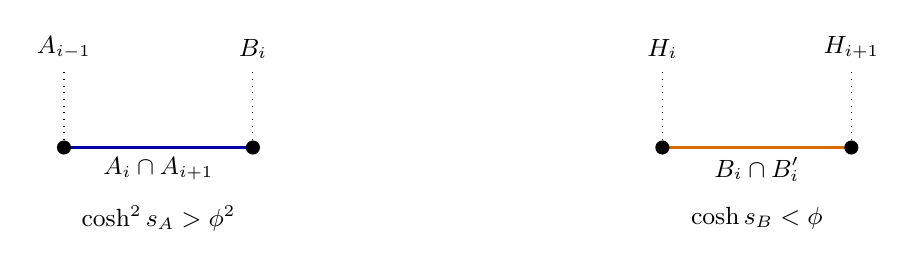
\begin{tikzpicture}[x=1cm,y=1cm,every node/.style={font=\small},
  vertex/.style={circle,fill=black,inner sep=1.8pt}]
 \begin{scope}[xshift=-3.8cm]
  \draw[very thick,blue!65!black] (-1.2,0)--(1.2,0);
  \node[vertex] (u) at (-1.2,0) {};
  \node[vertex] (v) at (1.2,0) {};
  \draw[dotted] (u)--(-1.2,1) (v)--(1.2,1);
  \node[above] at (-1.2,1) {$A_{i-1}$};
  \node[above] at (1.2,1) {$B_i$};
  \node[below] at (0,0) {$A_i\cap A_{i+1}$};
  \node at (0,-.9) {$\cosh^2s_A>\phi^2$};
 \end{scope}
 \begin{scope}[xshift=3.8cm]
  \draw[very thick,orange!85!black] (-1.2,0)--(1.2,0);
  \node[vertex] (u) at (-1.2,0) {};
  \node[vertex] (v) at (1.2,0) {};
  \draw[dotted] (u)--(-1.2,1) (v)--(1.2,1);
  \node[above] at (-1.2,1) {$H_i$};
  \node[above] at (1.2,1) {$H_{i+1}$};
  \node[below] at (0,0) {$B_i\cap B'_i$};
  \node at (0,-.9) {$\cosh s_B<\phi$};
 \end{scope}
\end{tikzpicture}
\caption{The two C26 witness edges and their endpoint third walls.
The incidence labels identify actual edges in the displayed dual
triangulation. One edge is longer and the other shorter than the
regular-pentagon edge; the drawings do not prescribe a Euclidean metric.}
\label{fig:c26-witnesses}
\end{figure}

\subsection{The twenty-eight-vertex cases}

\begin{proposition}\label{prop:c28}
A compact right-angled three-polyhedron with $28$ vertices contains no
regular pentagonal face.
\end{proposition}
\begin{proof}
There are $42$ edges and $16$ faces. Polygon capacity permits sizes at
most seven. A heptagon attains equality, so the full equality argument
after Lemma~\ref{lem:polygon} gives $L_7$. Metric uniqueness realizes
its base rotation, and every lateral pentagon has a base edge of cosh
\[
 1+2\cos(2\pi/7)>1+2\cos(2\pi/5)=\phi.
\]
It is not regular. Otherwise all faces are pentagons or hexagons:
twelve pentagons and four hexagons. We exhibit the two fullerene types
and treat their metrics separately.

\paragraph{The tetrahedral type.}
Use four labels $i=0,1,2,3$. The dual vertices are $H_i$ and $P_{ij}$
for $i\ne j$. Begin with the truncated tetrahedron on the twelve
directed-edge labels $P_{ij}$. Retain its four triangles
$\{P_{ij}:j\ne i\}$. For each remaining label $k$, with other labels
$i,j,l$, insert $H_k$ into the hexagon
\[
 P_{ij},P_{ji},P_{jl},P_{lj},P_{li},P_{il}
\]
and join it to all six boundary vertices. This is a triangulated
sphere with $28$ triangles. The twelve $P$ vertices have degree five;
the four $H$ vertices have degree six. Every permutation of the four
labels is an automorphism, transitive on the twelve $P$-pentagons.

At the actual common fixed point from Lemma~\ref{lem:actual-symmetry},
the four spatial $H$ vectors have equal lengths and equal pair
products. Their Euclidean Gram has rank at most three. The rank-one
alternative would identify the actual normals, so they are regular
tetrahedral directions $v_i$, with $v_i\cdot v_j=-1/3$ for $i\ne j$.
The stabilizer of an ordered pair fixes exactly the plane of $v_i,v_j$.
The actual normals therefore have the form
\[
 H_i=(h,-Rv_i),\qquad P_{ij}=(a,Av_i+Bv_j),\qquad R^2=1+h^2.
\]
Orthogonality to the two $H_k$ with $k\ne i,j$ gives $A+B=3ah/R>0$.
The adjacent pairs $P_{ij}P_{ik}$ and $P_{ij}P_{ji}$ give
\[
 a^2=A^2-\frac{2AB+B^2}{3}
     =2AB-\frac{A^2+B^2}{3}.
\]
The unit norm then gives $B^2=3/4$, and subtraction gives
$A(A-2B)=0$. The branch $A=0$ makes $a^2<0$, so $A=2B$ and $B>0$.
It follows that $a^2=7/4$, $h^2=3/4$ and $R^2=7/4$. The actual edge
$P_{ij}\cap P_{ji}$ has endpoint third walls $H_k,H_l$ for the other
two indices. Thus its cosh length is
\[
 h^2+R^2/3=4/3<\phi.
\]
Every pentagon contains such an edge, resolving this type.

\paragraph{The second type.}
Its dual labels are $H_0,H_1,H_2,H_3$ and
$A,B,C,D,E,F,G,J,K,M,N,P$. The triangles are
\begin{center}\small
\begin{tabular}{llll}
$H_0H_1A$&$H_0H_1B$&$H_0BC$&$H_0CD$\\
$H_0DE$&$H_0EA$&$AEF$&$AFG$\\
$AGH_1$&$H_1GJ$&$H_1JK$&$H_1KB$\\
$BKM$&$BMC$&$CMN$&$CND$\\
$DNH_2$&$DH_2E$&$EH_2F$&$H_2FP$\\
$FGP$&$GJP$&$JH_3P$&$JKH_3$\\
$KMH_3$&$MNH_3$&$NH_2H_3$&$H_2H_3P$.
\end{tabular}
\end{center}
Every edge has two incidences. The complete cyclic links are
\begin{center}\small
\begin{tabular}{ll@{\qquad}ll}
$H_0$&$H_1,B,C,D,E,A$&$H_1$&$H_0,B,K,J,G,A$\\
$H_2$&$D,E,F,P,H_3,N$&$H_3$&$J,K,M,N,H_2,P$\\
$A$&$H_0,E,F,G,H_1$&$B$&$H_0,C,M,K,H_1$\\
$C$&$H_0,D,N,M,B$&$D$&$H_0,E,H_2,N,C$\\
$E$&$H_0,A,F,H_2,D$&$F$&$A,G,P,H_2,E$\\
$G$&$A,H_1,J,P,F$&$J$&$H_1,K,H_3,P,G$\\
$K$&$H_1,B,M,H_3,J$&$M$&$B,C,N,H_3,K$\\
$N$&$C,D,H_2,H_3,M$&$P$&$F,G,J,H_3,H_2$.
\end{tabular}
\end{center}
These links and connectedness give a closed surface, and
$16-42+28=2$ gives a sphere. The $H$-induced graph has two edges,
$H_0H_1,H_2H_3$, whereas the tetrahedral type has none. The two spheres
are therefore nonisomorphic. Together with the published count two,
this proves exhaustiveness of the fullerene branch.

The commuting involutions
\[
 \begin{split}
 \alpha={}&(H_0\ H_1)(H_2\ H_3)(A\ B)(C\ G)
                  (D\ J)(E\ K)(F\ M)(N\ P),\\
 \beta={}&(H_0\ H_2)(H_1\ H_3)(A\ N)(B\ P)
                  (C\ F)(D\ E)(G\ M)(J\ K)
 \end{split}
\]
preserve every triangle. Their pentagon orbits are
\[
 \{A,B,N,P\},\qquad \{D,E,J,K\},\qquad \{C,F,G,M\}.
\]
They act by actual isometries of an assumed polyhedron of this type.
If a face in the first orbit is regular, all four are regular, and
$C$ has two $L$-edges from its neighbors $B,N$. By
Lemma~\ref{lem:any-two-pentagon}, the third orbit is regular too.
If instead the third orbit is initially regular, $A$ has two $L$-edges
from $F,G$, reducing to that case. Once both outer orbits are regular,
$D$ has two $L$-edges from $C,N$, making the middle orbit regular.
All twelve pentagons would be regular. The hexagon $H_0$ then has
five consecutive $L$-edges, contrary to Lemma~\ref{lem:three-edges}.
Thus only the middle orbit could contain a regular pentagon.

Assume that orbit is regular. We again use face labels for actual
outward unit normals. The orthogonal $D,E$ are both orthogonal to
$H_0,H_2$, and regularity of $D$ gives $\ip{H_0}{H_2}=-\phi$.
Thus $D,E,H_0,H_2$ are a nondegenerate Lorentz basis. The nonadjacent
side normals of a regular pentagon have product $-\phi$. Reading the
links of $D,E$ determines
\begin{equation}\label{eq:c28-AC}
 A=-\phi D+\phi H_0+H_2,\qquad
 C=-\phi E+\phi H_0+H_2.
\end{equation}
For example $A$ has products $0$ with $E,H_0$ and $-\phi$ with
$D,H_2$; these four products give its unique coordinates.

Put $\ip{H_0}{H_3}=\ip{H_1}{H_2}=-k$, the equality following from
$\alpha$, and put $e=\ip{H_1}E$. Nonadjacency gives $k>1$.
The other $H$ products are
\[
 \ip{H_0}{H_1}=\ip{H_2}{H_3}=0,
 \qquad \ip{H_1}{H_3}=-\phi.
\]
The last equality follows from the regular pentagon $J$.
Since $\ip A{H_1}=0$, equation~\eqref{eq:c28-AC} gives
\[
 H_1=-\frac{k}{\phi}D+eE+kH_0+\frac{k}{\phi}H_2.
\]
Apply $\beta$ to obtain $H_3$. Unit norm and the product
$\ip{H_1}{H_3}=-\phi$ give
\[
 e^2=1+\phi^{-3}k^2,\qquad
 e=\frac{\phi-k^2}{2\phi^{-1}k}.
\]
Using $\phi^2=\phi+1$, elimination yields
\[
 (33-20\phi)k^4-(8-2\phi)k^2+\phi^2=0.
\]
Its roots in $k^2$ are $\phi^4$ and $(6+7\phi)/29$; multiplication
recovers the displayed quadratic, whose leading coefficient is positive.
The second root is below one, so $k=\phi^2$ and $e=-\phi$.
Finally~\eqref{eq:c28-AC} gives
\[
 \ip C{H_1}=-\phi e-k=0.
\]
But $C,H_1$ are nonadjacent in the displayed link table. The actual
orthogonal-wall intersection lemma makes this impossible. This resolves
the remaining orbit, the second fullerene and the proposition.
\end{proof}

\begin{figure}[tb]
\centering
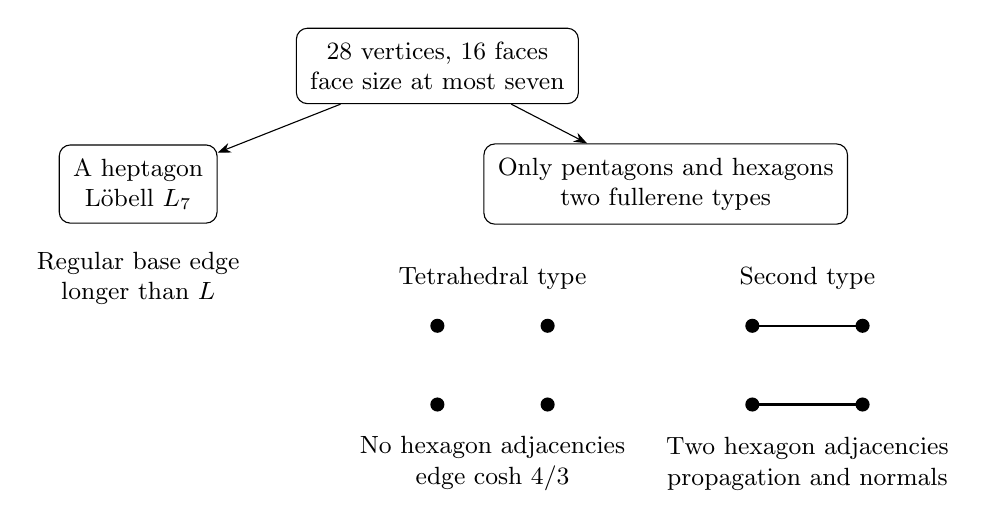
\begin{tikzpicture}[every node/.style={font=\small},
 box/.style={draw,rounded corners,align=center,inner sep=5pt},
 dot/.style={circle,fill=black,inner sep=1.8pt}]
 \node[box] (start) at (0,2.6) {$28$ vertices, $16$ faces\\face size at most seven};
 \node[box] (seven) at (-3.8,1.1) {A heptagon\\L\"obell $L_7$};
 \node[box] (six) at (2.9,1.1) {Only pentagons and hexagons\\two fullerene types};
 \draw[-{Stealth}] (start)--(seven);
 \draw[-{Stealth}] (start)--(six);
 \node[align=center] at (-3.8,-.1) {Regular base edge\\longer than $L$};
 \node at (.7,-.1) {Tetrahedral type};
 \node at (4.7,-.1) {Second type};
 \foreach \x/\y in {0/.0,1.4/.0,0/-1.0,1.4/-1.0}{
   \node[dot] at (\x,\y-.7) {};}
 \foreach \x/\y in {4/.0,5.4/.0,4/-1.0,5.4/-1.0}{
   \node[dot] at (\x,\y-.7) {};}
 \draw[thick] (4,-.7)--(5.4,-.7) (4,-1.7)--(5.4,-1.7);
 \node[align=center] at (.7,-2.45) {No hexagon adjacencies\\edge cosh $4/3$};
 \node[align=center] at (4.7,-2.45) {Two hexagon adjacencies\\propagation and normals};
\end{tikzpicture}
\caption{The exhaustive C28 branch. The lower diagrams show only the
subgraphs on the four hexagonal faces. Their different edge counts
distinguish the two fullerene types; the full dual spheres are specified
in the proof. Each branch excludes an entire regular pentagonal face.}
\label{fig:c28-branches}
\end{figure}

\section{The whole-polytope lower bound}

\begin{proof}[Proof of Theorem~\ref{thm:global-lower}]
Theorem~\ref{thm:farthest-dodecahedron} supplies a regular dodecahedral
facet $D$. If every facet is dodecahedral, Proposition~\ref{prop:zero}
gives the regular $120$-cell, which satisfies the stated bounds.
Otherwise connected facet adjacency supplies a positive facet $Q$
adjacent to some dodecahedral facet. Their shared ridge is an entire
regular pentagon.

Lemma~\ref{lem:small-degree} excludes excess one. An excess-two facet
has two unit nonpentagonal edges and hence is $L_6$; its lateral
pentagons have a base edge of cosh $2$, so none is regular. Excess
three gives $26$ vertices and is excluded by Proposition~\ref{prop:c26};
excess four gives $28$ vertices and is excluded by
Proposition~\ref{prop:c28}. Therefore $d(Q)\ge5$ and $V(Q)\ge30$.
Facet capacity yields $f\ge2\cdot30+5=65$.

In the non-all-dodecahedral case, Theorem~\ref{thm:gap} also gives
$W\ge17$. The exact volume identity gives
\[
 \Vol(P)\ge\frac{\pi^2}{12}(65+17+16)=\frac{49\pi^2}{6}.
\]
The all-dodecahedral case has volume $34\pi^2/3$, so the same
inequality holds there too.
\end{proof}

\section{Finite verification and proof boundaries}\label{sec:verification}

The proofs above begin with actual compact polyhedra. The finite
classification is the published count-one/count-two statement, not a
search carried out by our scripts. Once those counts are supplied, it
suffices to identify the fixed dual spheres and verify the displayed
metric consequences. The companion checks make this finite arithmetic
reproducible without replacing its geometric interpretation.

For a prescribed triangle list, form its complete edge-incidence map.
Check two triangles per edge, connectedness, and a connected degree-two
link at every vertex; then check Euler characteristic two and the stated
five/six degree counts. These conditions prove that the complex is a
triangulated sphere with the required fullerene dual. A permutation is
an automorphism exactly when it preserves the entire triangle set.
The C26 check closes the three specified generators to twelve
permutations; the tetrahedral C28 check tests all $24$ label permutations;
the second C28 check tests the four specified permutations and all three
orbits. The regular-pentagon propagation repeatedly enlarges a subset of
twelve labels and therefore halts after at most twelve strict enlargements.
All graph loops are over these explicit finite lists. They do not claim
to enumerate the fullerene classification itself.

For the metric identities, represent a number by the rational pair
$(a,b)$ meaning $a+b\sqrt d$, with $d=17$ or $5$. Addition and
multiplication use rational arithmetic; inversion uses
$(a-b\sqrt d)/(a^2-db^2)$. For opposite coefficient signs, the sign is
decided by comparing $a^2$ and $db^2$; for equal signs it is immediate.
The positive square root specifies the physical embedding. Binary
exponentiation decreases its exponent, and the determinant recurrence
decreases matrix order. Thus these exact checks halt and test every
listed identity, without numerical tolerances or an angle cutoff.

The retained C26 output has $15$ dual vertices, $39$ edges, $26$
triangles and order $12$ for the generated action. Its two witness values are
$(7+\sqrt{17})/4$ for the squared cosh and $(1+\sqrt{17})/4$ for the
cosh. The C28 output checks both $(16,42,28)$ dual spheres, the
$24$- and $4$-element actions, the two-orbit propagation and the
quartic factorization above. The older C28 certificate also checks the
longer two-unit-normal-fiber contradiction; the main proof uses its
shorter actual-adjacency consequence.

Generation and a separate fresh-process replay have been recorded for
each fixed checker. They compare the complete returned certificate,
not only a final scalar. Those runs supply fixed graph and exact
algebra evidence. They do not establish metric uniqueness, actual
incidence from arbitrary Gram data, the published counts, Gauss--Bonnet,
or the universal W-gap proof. The source ledger for this draft identifies
the exact inputs, checks and preserved executions. A separate source-bound review of this consolidated translation records
its mathematical acceptance. The earlier executions retain their original
fixed-model scopes; PDF compilation and conditional formalization have
separate verification records.

\section{Remaining volume questions}

The remaining minimum-volume target is $f+W\ge120$. The present lower
bound gives $f\ge65$ and, outside the $120$-cell, $W\ge17$; it does
not reach that target. A competing polytope at or below the $120$-cell
volume must also have at most $46$ vertices in each facet. These local
restrictions do not classify its larger positive facets or their global
compatibility. Below the reflected double the corresponding cutoff is
$96$, and no second-volume gap or equality theorem follows.

No center-cut, inball or homology refinement is used in this paper.
The fixed algebraic models do not assume arithmeticity, and no assertion
that arbitrary compact right-angled four-polytopes decompose into regular
$120$-cells enters any proof. The geometric, topological and published
classification interfaces remain explicit; conditional Lean kernels do
not constitute an end-to-end formalization of them.
\begin{thebibliography}{9}
\bibitem{AVS}
D.~V.~Alekseevskij, E.~B.~Vinberg and A.~S.~Solodovnikov,
\emph{Geometry of spaces of constant curvature}, in
\emph{Geometry II}, Encyclopaedia of Mathematical Sciences~29,
Springer, 1993, pp.~1--138.

\bibitem{PV}
L.~Potyagailo and E.~Vinberg,
\emph{On right-angled reflection groups in hyperbolic spaces},
Commentarii Mathematici Helvetici~80 (2005), 63--73.
\url{https://ems.press/content/serial-article-files/43032}.

\bibitem{KP}
R.~Kellerhals and G.~Perren,
\emph{On the growth of cocompact hyperbolic Coxeter groups},
European Journal of Combinatorics~32 (2011), 1299--1316.
\url{https://doi.org/10.1016/j.ejc.2011.03.020}.

\bibitem{Inoue}
T.~Inoue, \emph{Organizing volumes of right-angled hyperbolic polyhedra},
Algebraic \& Geometric Topology~8 (2008), 1523--1565.
\url{https://doi.org/10.2140/agt.2008.8.1523}.

\bibitem{KK}
R.~Kellerhals and A.~Kolpakov,
\emph{The minimal growth rate of cocompact Coxeter groups in hyperbolic
three-space}, Canadian Journal of Mathematics~66 (2014), 354--372.
\url{https://homeweb.unifr.ch/kellerha/pub/CJM-KellKolp-J0844-FINAL.pdf}.

\bibitem{ABVE}
S.~A.~Alexandrov, N.~V.~Bogachev, A.~Yu.~Vesnin and A.~A.~Egorov,
\emph{On volumes of hyperbolic right-angled polyhedra},
Sbornik: Mathematics~214 (2023), 148--165.
\url{https://doi.org/10.4213/sm9740e}.

\bibitem{BGM}
G.~Brinkmann, J.~Goedgebeur and B.~D.~McKay,
\emph{The generation of fullerenes}, Journal of Chemical Information
and Modeling~52 (2012), 2910--2918; author's accepted version,
Table~2, PDF p.~15.
\url{https://arxiv.org/pdf/1207.7010v2}.

\bibitem{RHD}
R.~K.~W.~Roeder, J.~H.~Hubbard and W.~D.~Dunbar,
\emph{Andreev's theorem on hyperbolic polyhedra},
Annales de l'Institut Fourier~57 (2007), 825--882.
\url{https://doi.org/10.5802/aif.2279}.
\end{thebibliography}
\end{document}
